\documentclass[dvisvgm,tikz]{standalone}
\begin{document}
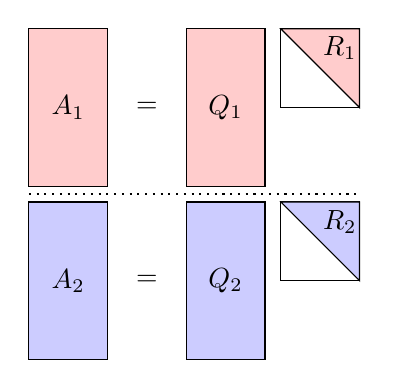
\begin{tikzpicture}

\filldraw[fill=red!20] (0,2.2) rectangle (1,4.2);
\filldraw[fill=blue!20] (0,0) rectangle (1,2);
\node at (0.5,3.2) {$A_1$};
\node at (0.5,1) {$A_2$};
\filldraw[fill=red!20] (2,2.2) rectangle (3,4.2);
\filldraw[fill=blue!20] (2,0) rectangle (3,2);
\node at (2.5,3.2) {$Q_1$};
\node at (2.5,1) {$Q_2$};
\draw (3.2,3.2) rectangle (4.2,4.2);
\draw (3.2,1) rectangle (4.2,2);
\filldraw[fill=red!20] (3.2,4.2) -- (4.2,3.2) -- (4.2,4.2) -- cycle;
\filldraw[fill=blue!20] (3.2,2) -- (4.2,1) -- (4.2,2) -- cycle;
\node at (3.95,3.95) {$R_1$};
\node at (3.95,1.75) {$R_2$};

\node at (1.5,1) {$=$};
\node at (1.5,3.2) {$=$};

\draw[thick,dotted] (0,2.1) -- (4.2,2.1);

\end{tikzpicture}
\end{document}
